\section{Results}
\label{Results}
\subsection{\psitwos-to-\jpsi ratio as function of $N^{\rm PV}_{\rm tracks}$}
The \psitwos-to-\jpsi production ratio is measured as function of $N^{\rm PV}_{\rm tracks}$, as shown in Fig~\ref{RPVN} and summarized in Sec~\ref{Table of ratios}. The from-$b$ production ratio does not show dependence on $N^{\rm PV}_{\rm tracks}$ in both configurations. Prompt production ratio shows a decreasing trend with $N^{\rm PV}_{\rm tracks}$ in $p$Pb configuration, while no decreasing trend in $Pb$p configuration.
Then the relative modification of the ratio is normalized to the production ratio in $pp$ collisions by comparing the ratios in two systems. The double ratio as function of $N^{\rm PV}_{\rm tracks}$ is shown in Fig~\ref{RPVNpp}. Results shows that the suppression of \psitwos relative to the \jpsi in $p$Pb compared to $pp$ collisions appears to be stronger in the Pb-going direction (backward rapidity) where a higher mean value of multiplicity presents, while no clear trend of the ratio is observed. The result in $p$-going direction is compatible to that in $pp$ collisions, where the double ratio is around unit. The result agree with what has been observed by ALICE collaboration~\cite{ALICE:2020tsj}.
\begin{figure}[H]
  \begin{center}
    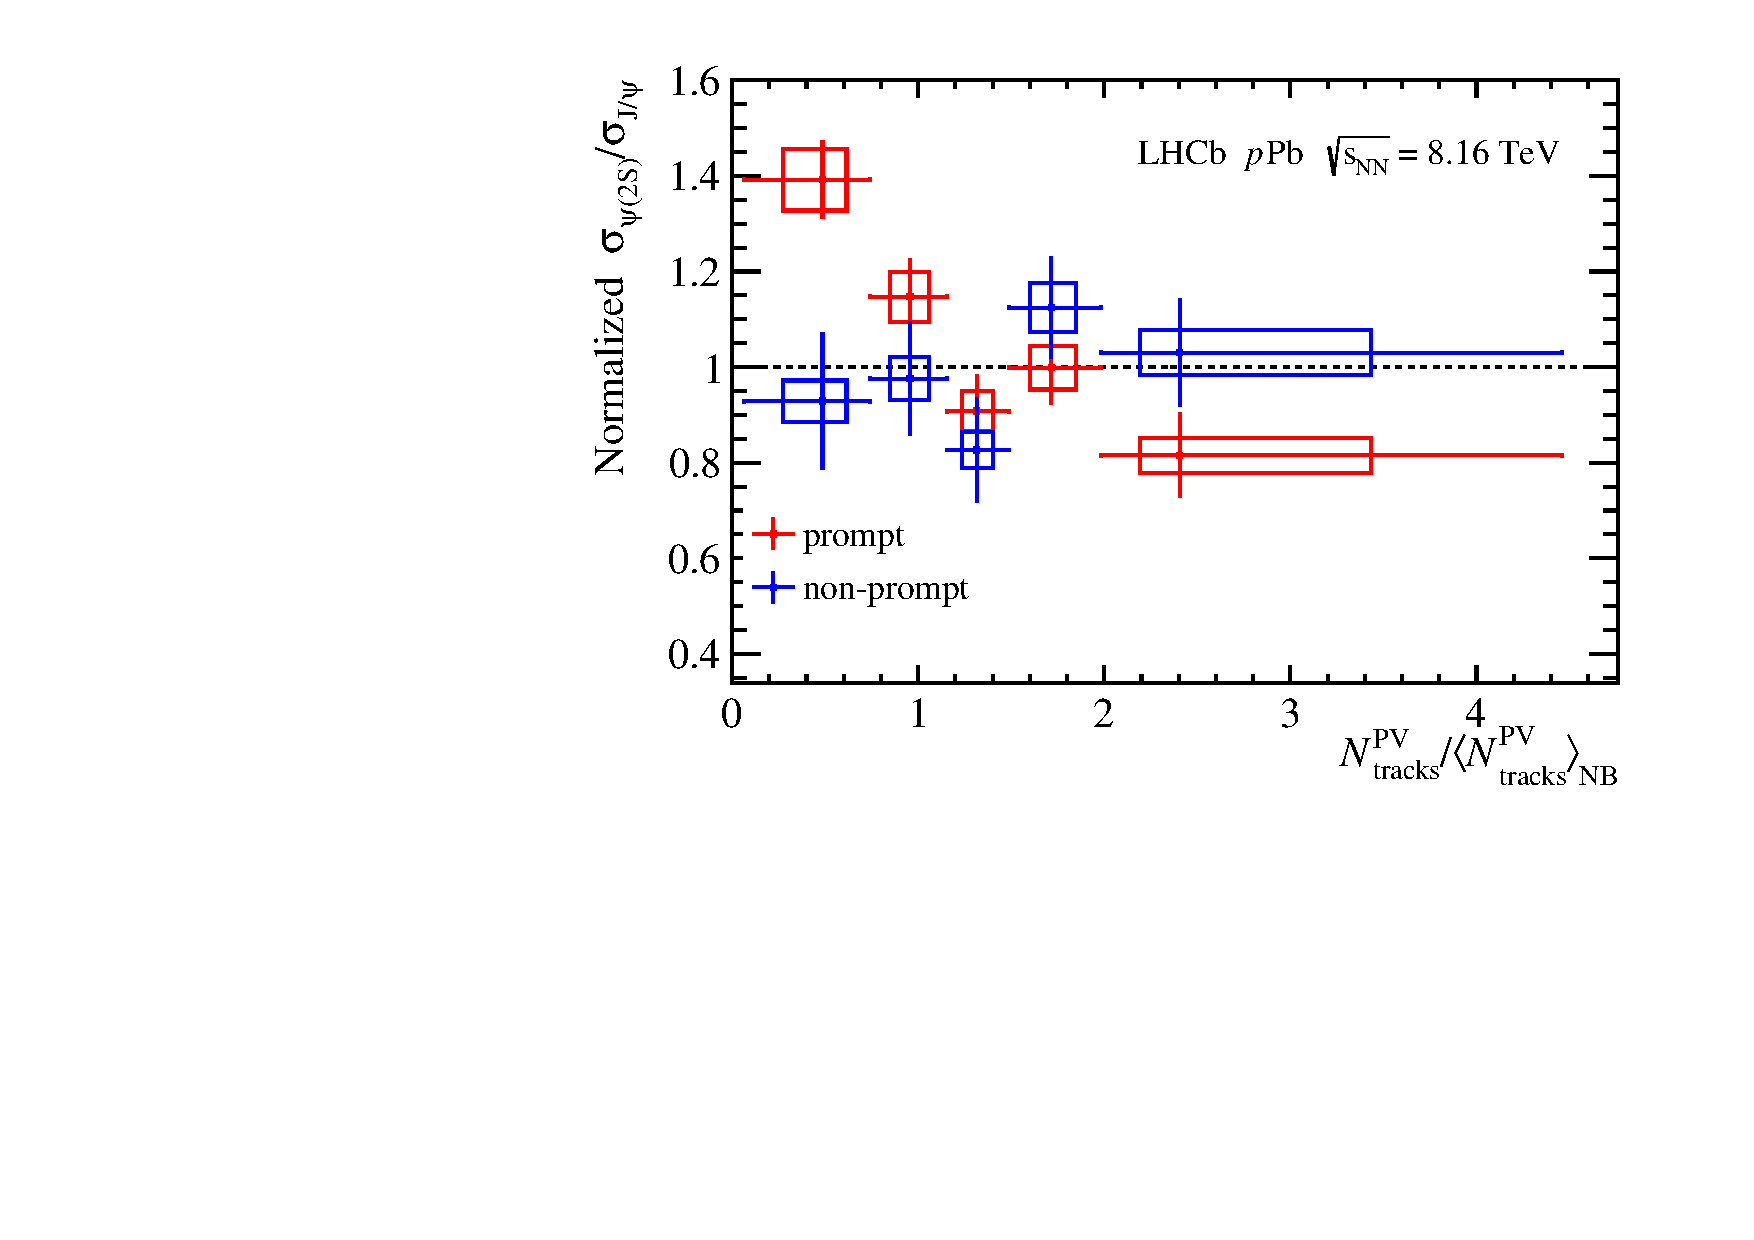
\includegraphics[width=0.49\linewidth]{pdf/pPb/Workdir/Result/All.pdf}
    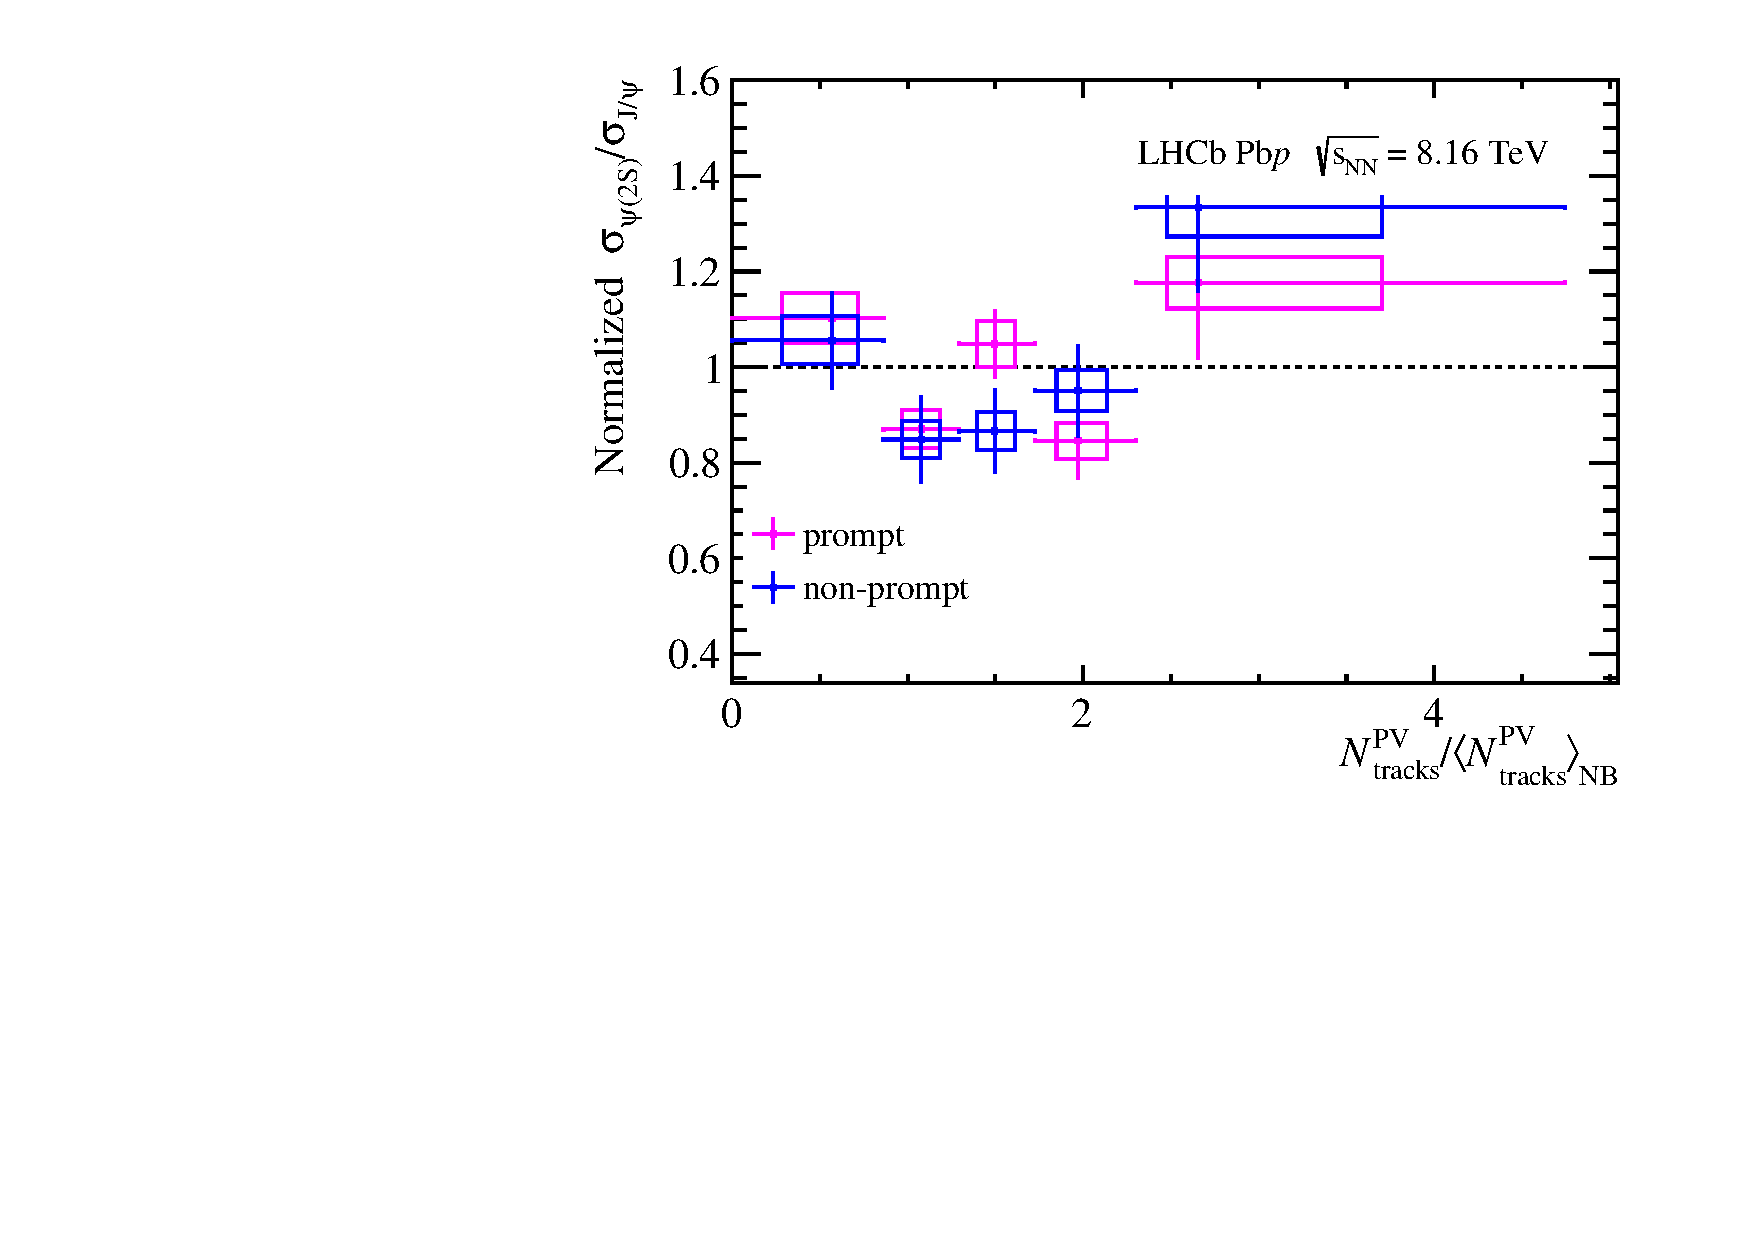
\includegraphics[width=0.49\linewidth]{pdf/Pbp/Workdir/Result/All.pdf}
    \vspace*{-0.5cm}
  \end{center}
  \caption{\psitwos-to-\jpsi production ratio as function of $N^{\rm PV}_{\rm tracks}$. The left is result in $p$Pb configuration and the right is in Pb$p$ configuration.
    }
  \label{RPVN}
\end{figure}

\begin{figure}[H]
    \begin{center}
	    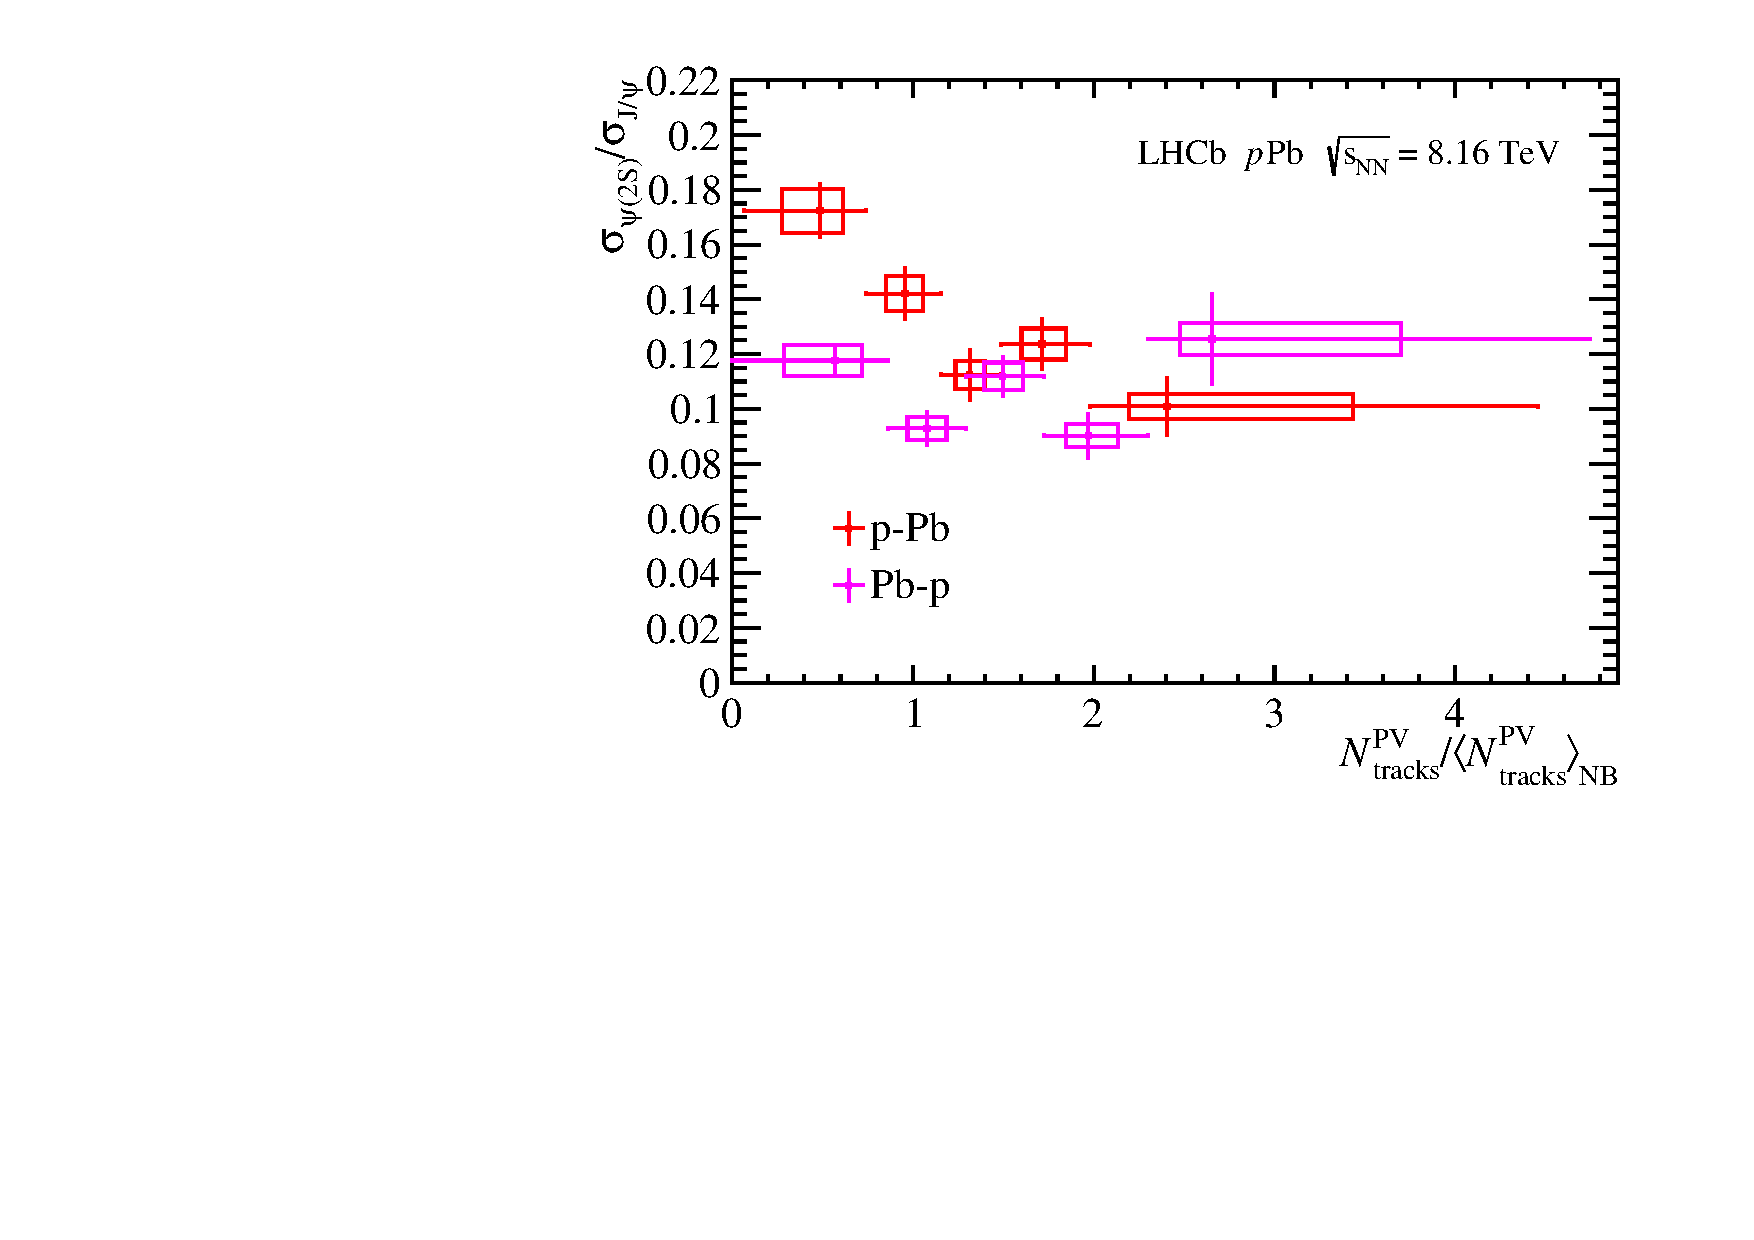
\includegraphics[width=0.7\linewidth]{pdf/pPb/Workdir/Result/Norm.pdf}
    \end{center}
    \caption{Prompt \psitwos-to-\jpsi production ratio compared with measurement in $pp$ collisions as a function of $N^{\rm PV}_{\rm tracks}$.
      }
    \label{RPVNpp}
\end{figure}
\subsection{\psitwos-to-\jpsi ratio as function of $N^{\rm PV}_{\rm fwd}$}
The \psitwos-to-\jpsi ratio as function of $N^{\rm PV}_{\rm fwd}$, which is measured in the same rapidity region of charmonia production, is presented in Fig~\ref{RFor} and Fig~\ref{RForpp}. The result is similar to what is observed in $N^{\rm PV}_{\rm tracks}$ scheme. No trend is observed for the from-$b$ production. For prompt production, the suppression of \psitwos relative to the \jpsi in $p$Pb compared to $pp$ collisions is stronger in the Pb-going direction, while no clear trend of the ratio is observed in Pb-going direction. The results shows a forward-backward asymmetry, where result in $p$-going direction is compatible to that in $pp$ collisions, and result in Pb-going direction shows clearly a different phenomenon to that in $pp$ collisions.
\begin{figure}[H]
  \begin{center}
    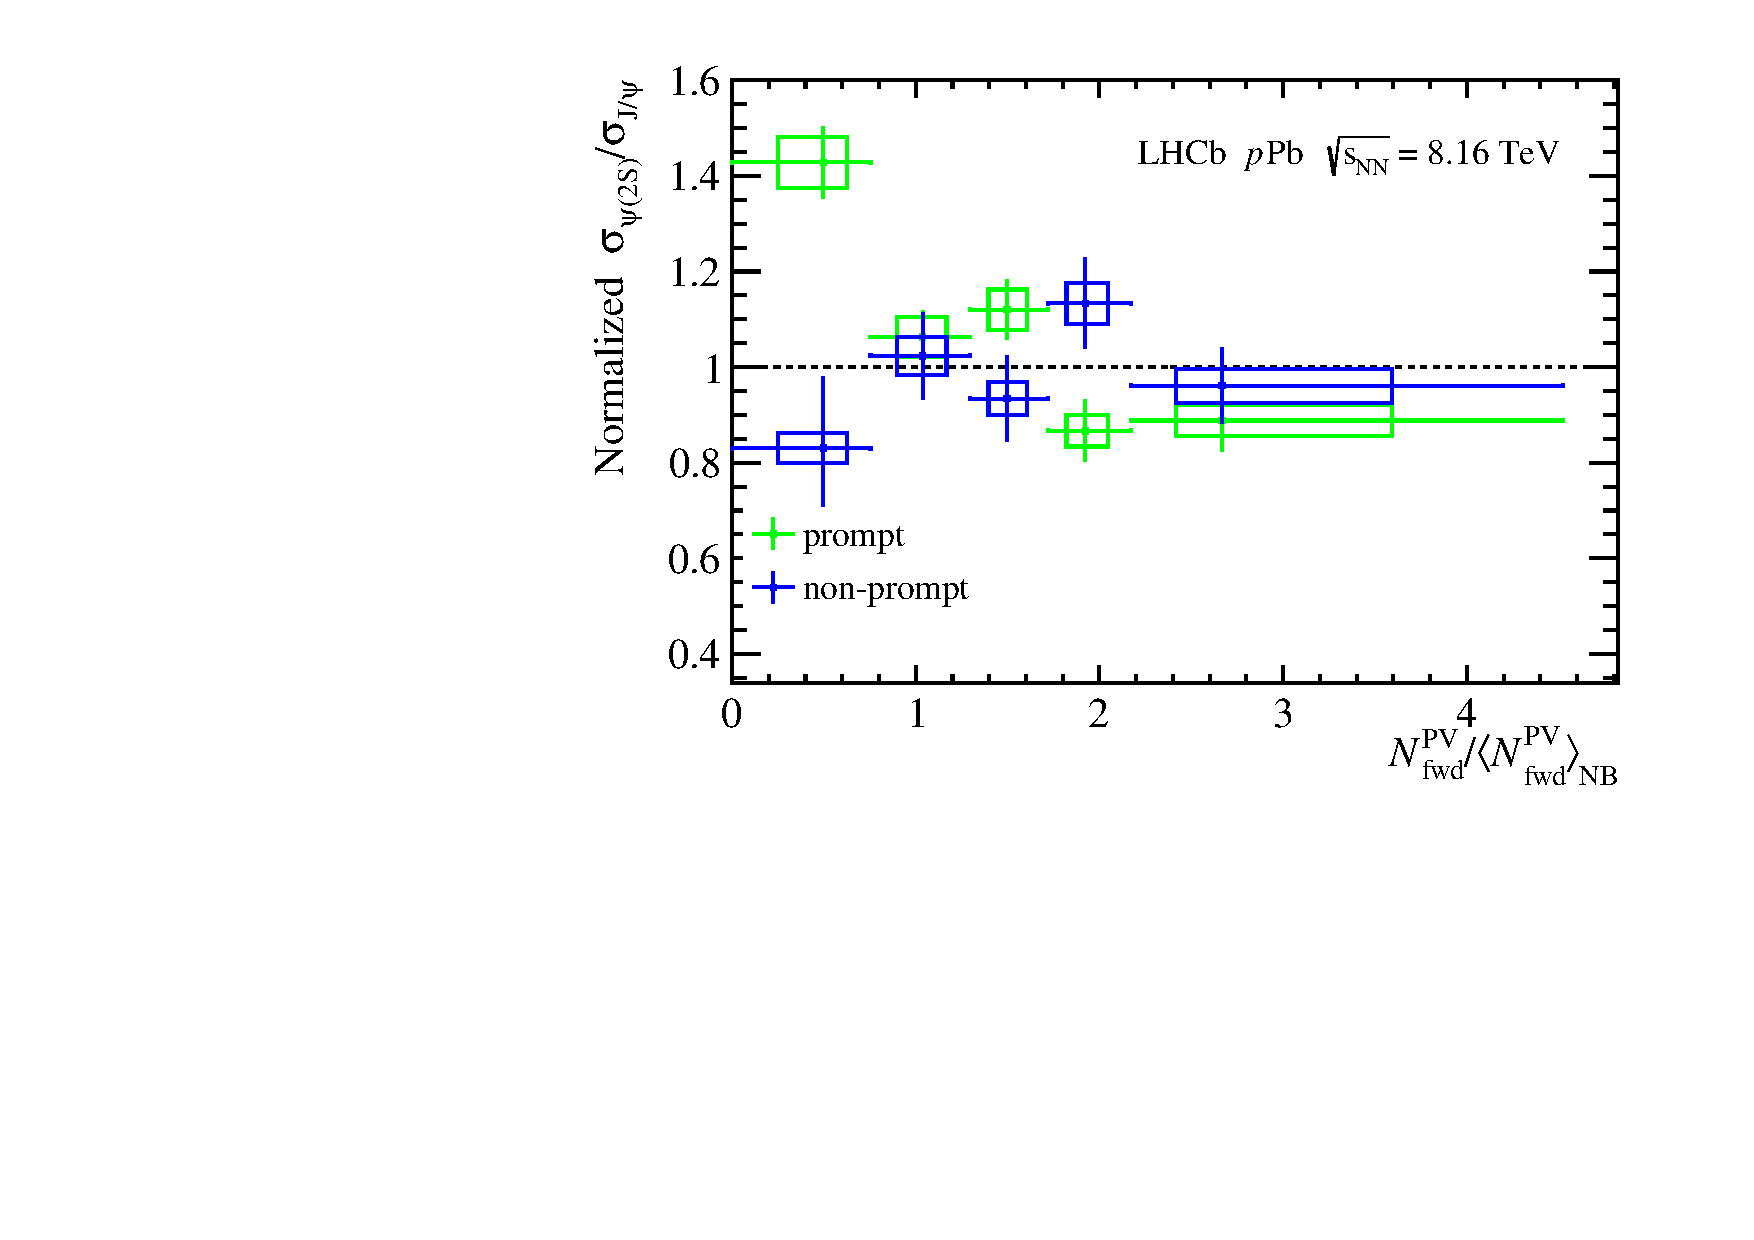
\includegraphics[width=0.49\linewidth]{pdf/pPb/FWorkdir/Result/All.pdf}
    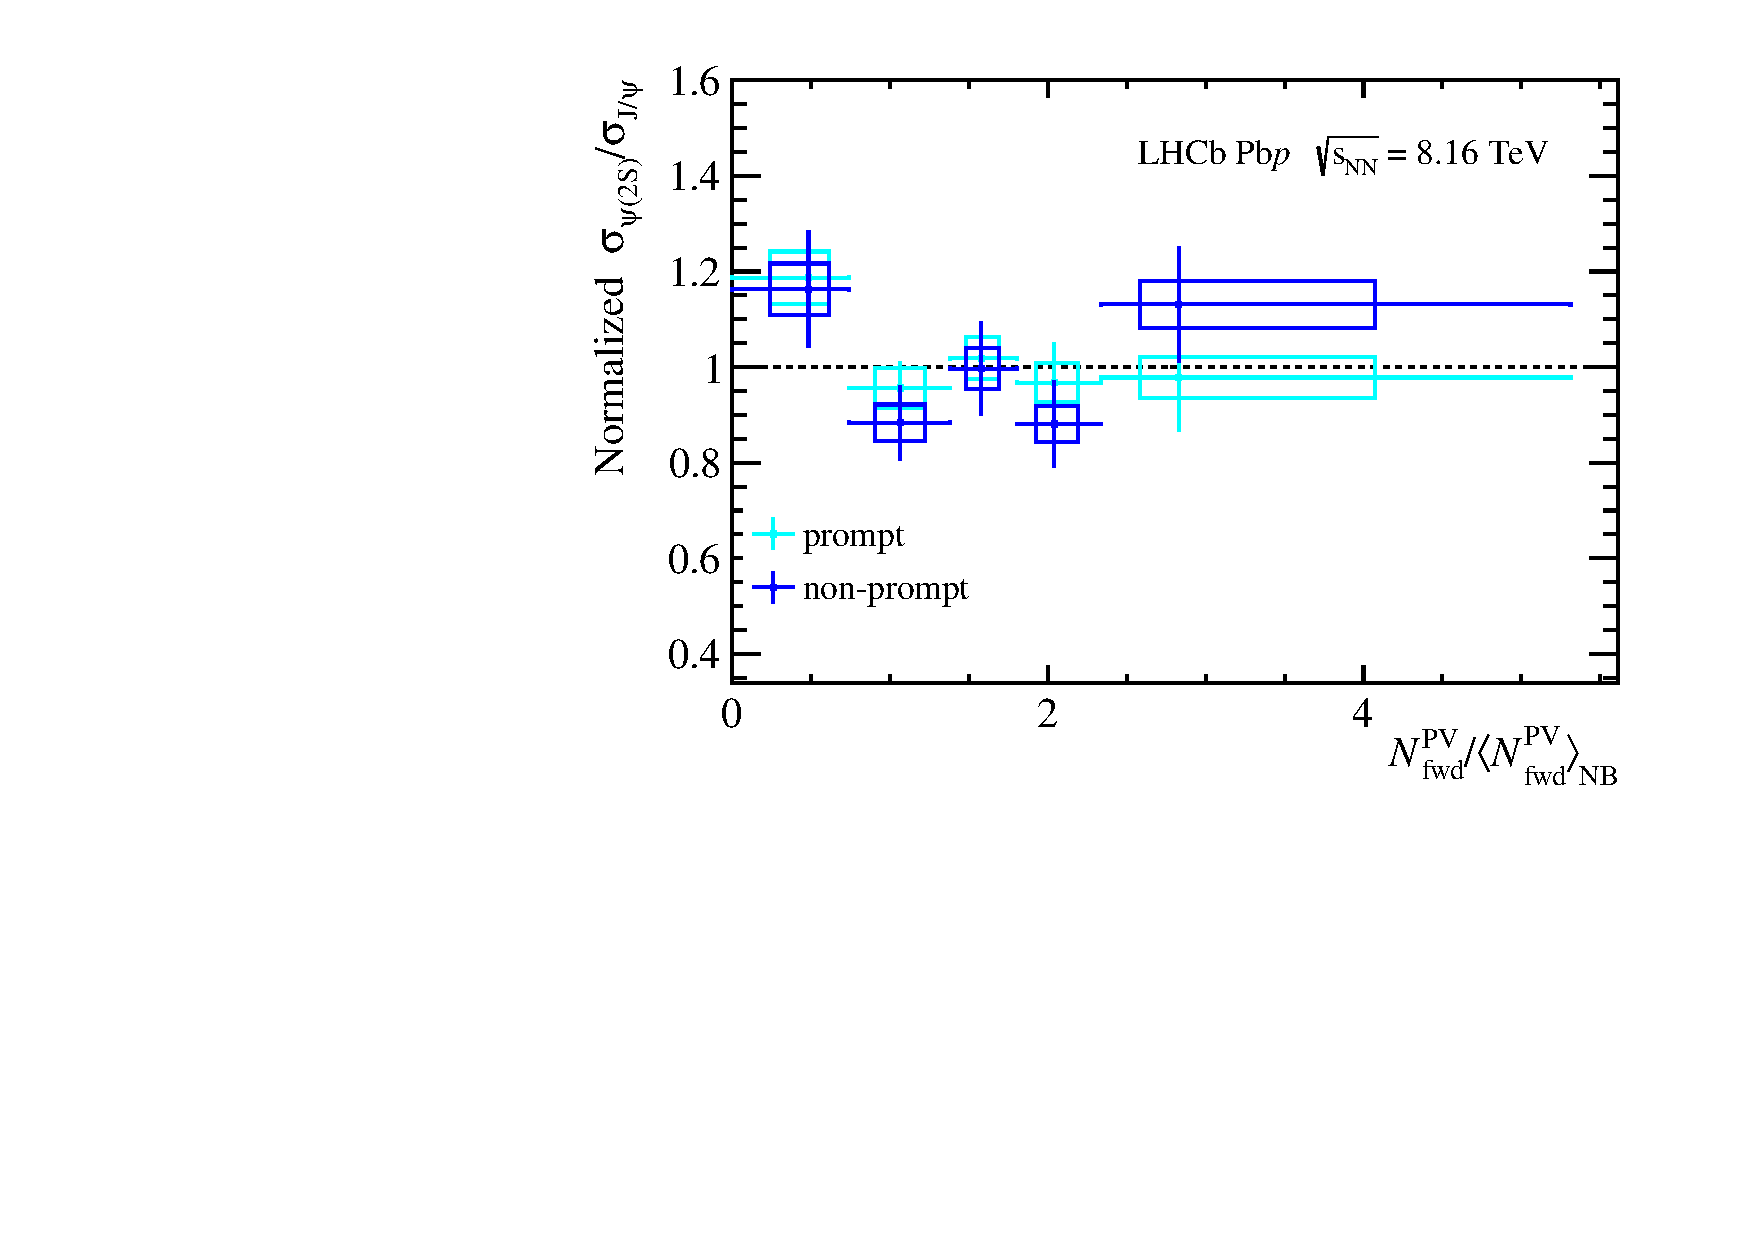
\includegraphics[width=0.49\linewidth]{pdf/Pbp/FWorkdir/Result/All.pdf}
    \vspace*{-0.5cm}
  \end{center}
  \caption{\psitwos-to-\jpsi production ratio as function of $N^{\rm PV}_{\rm fwd}$. The left is result in $p$Pb configuration and the right is in Pb$p$ configuration.
    }
  \label{RFor}
\end{figure}

\begin{figure}[H]
    \begin{center}
            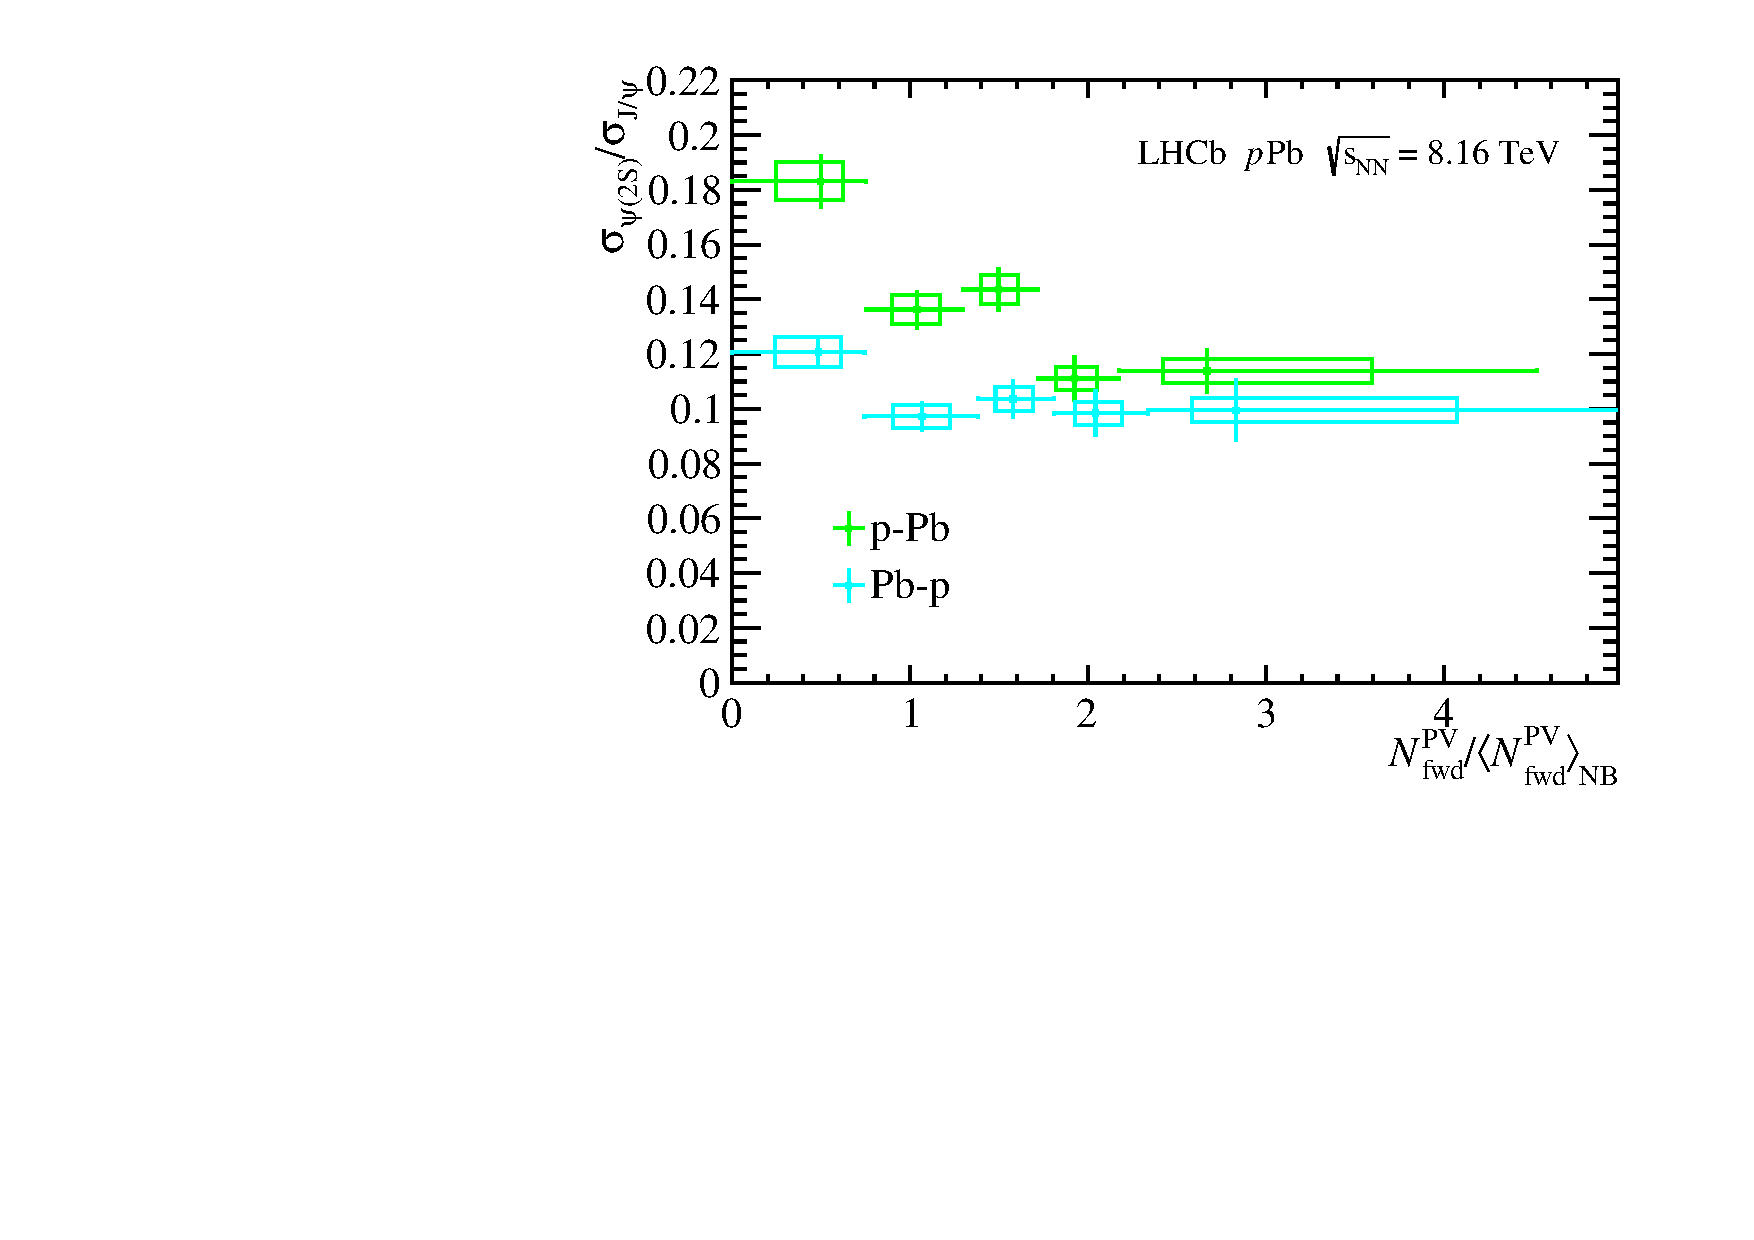
\includegraphics[width=0.7\linewidth]{pdf/pPb/FWorkdir/Result/Norm.pdf}
    \end{center}
    \caption{Prompt \psitwos-to-\jpsi production ratio compared with measurement in $pp$ collisions as a function of $N^{\rm PV}_{\rm fwd}$.
      }
    \label{RForpp}
\end{figure}
\subsection{\psitwos-to-\jpsi ratio as function of $N^{\rm PV}_{\rm bwd}$}
The ratio as function of $N^{\rm PV}_{\rm bwd}$ is shown in Fig~\ref{RBack} and Fig~\ref{RBackpp}. The use of $N^{\rm PV}_{\rm bwd}$, which is measured in the different rapidity range, allows us to reduce the correlation from charmonia production and multiplicity measurements. And within expectation, the decreasing trend \psitwos-to-\jpsi ratio in $p$Pb configuration almost vanishes compared to that in $N^{\rm PV}_{\rm tracks}$ and $N^{\rm PV}_{\rm fwd}$ schemes. Still,  the suppression of \psitwos relative to the \jpsi in $p$Pb compared to $pp$ collisions appears to be stronger in the Pb-going direction (backward rapidity),and no clear trend of the ratio is observed.
\begin{figure}[H]
  \begin{center}
    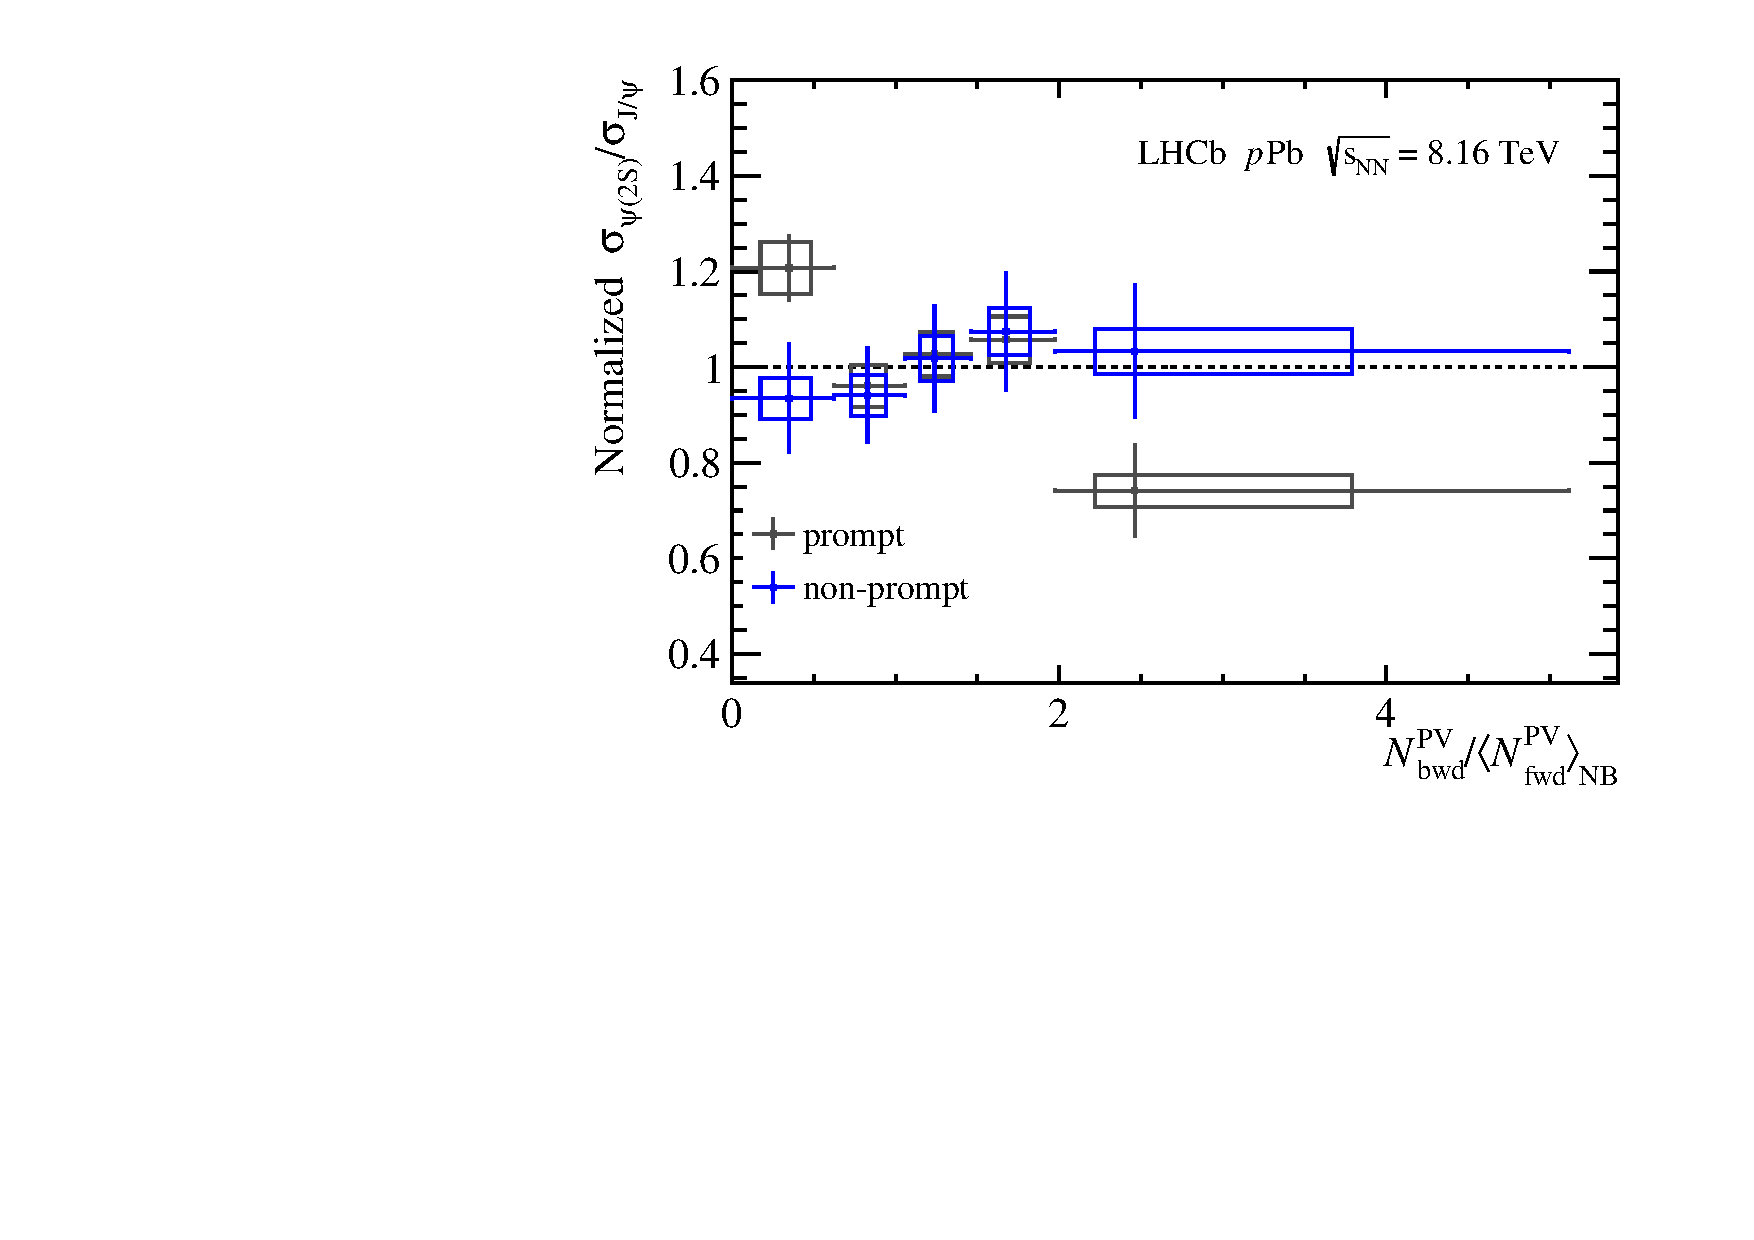
\includegraphics[width=0.49\linewidth]{pdf/pPb/BWorkdir/Result/All.pdf}
    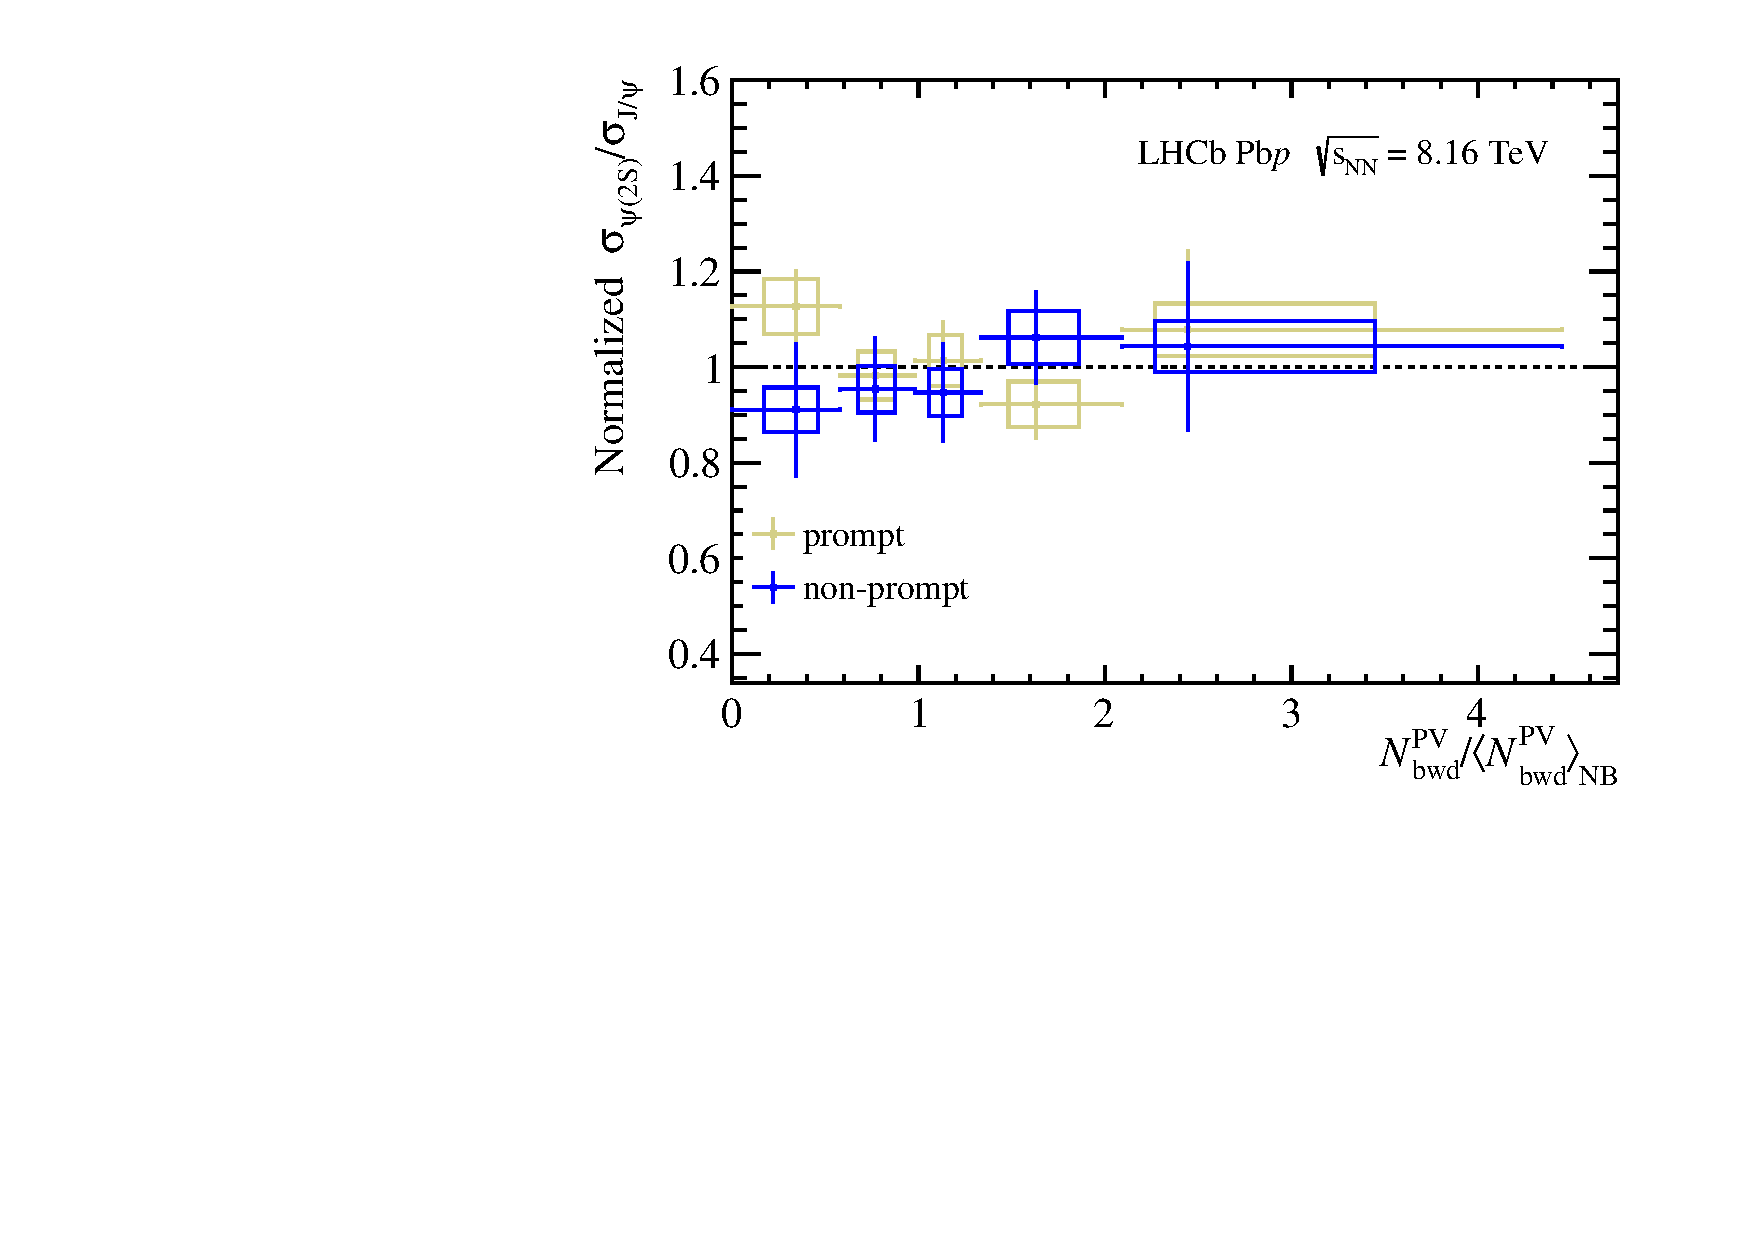
\includegraphics[width=0.49\linewidth]{pdf/Pbp/BWorkdir/Result/All.pdf}
    \vspace*{-0.5cm}
  \end{center}
  \caption{\psitwos-to-\jpsi production ratio as function of $N^{\rm PV}_{\rm bwd}$. The left is result in $p$Pb configuration and the right is in Pb$p$ configuration.
    }
  \label{RBack}
\end{figure}

\begin{figure}[H]
    \begin{center}
            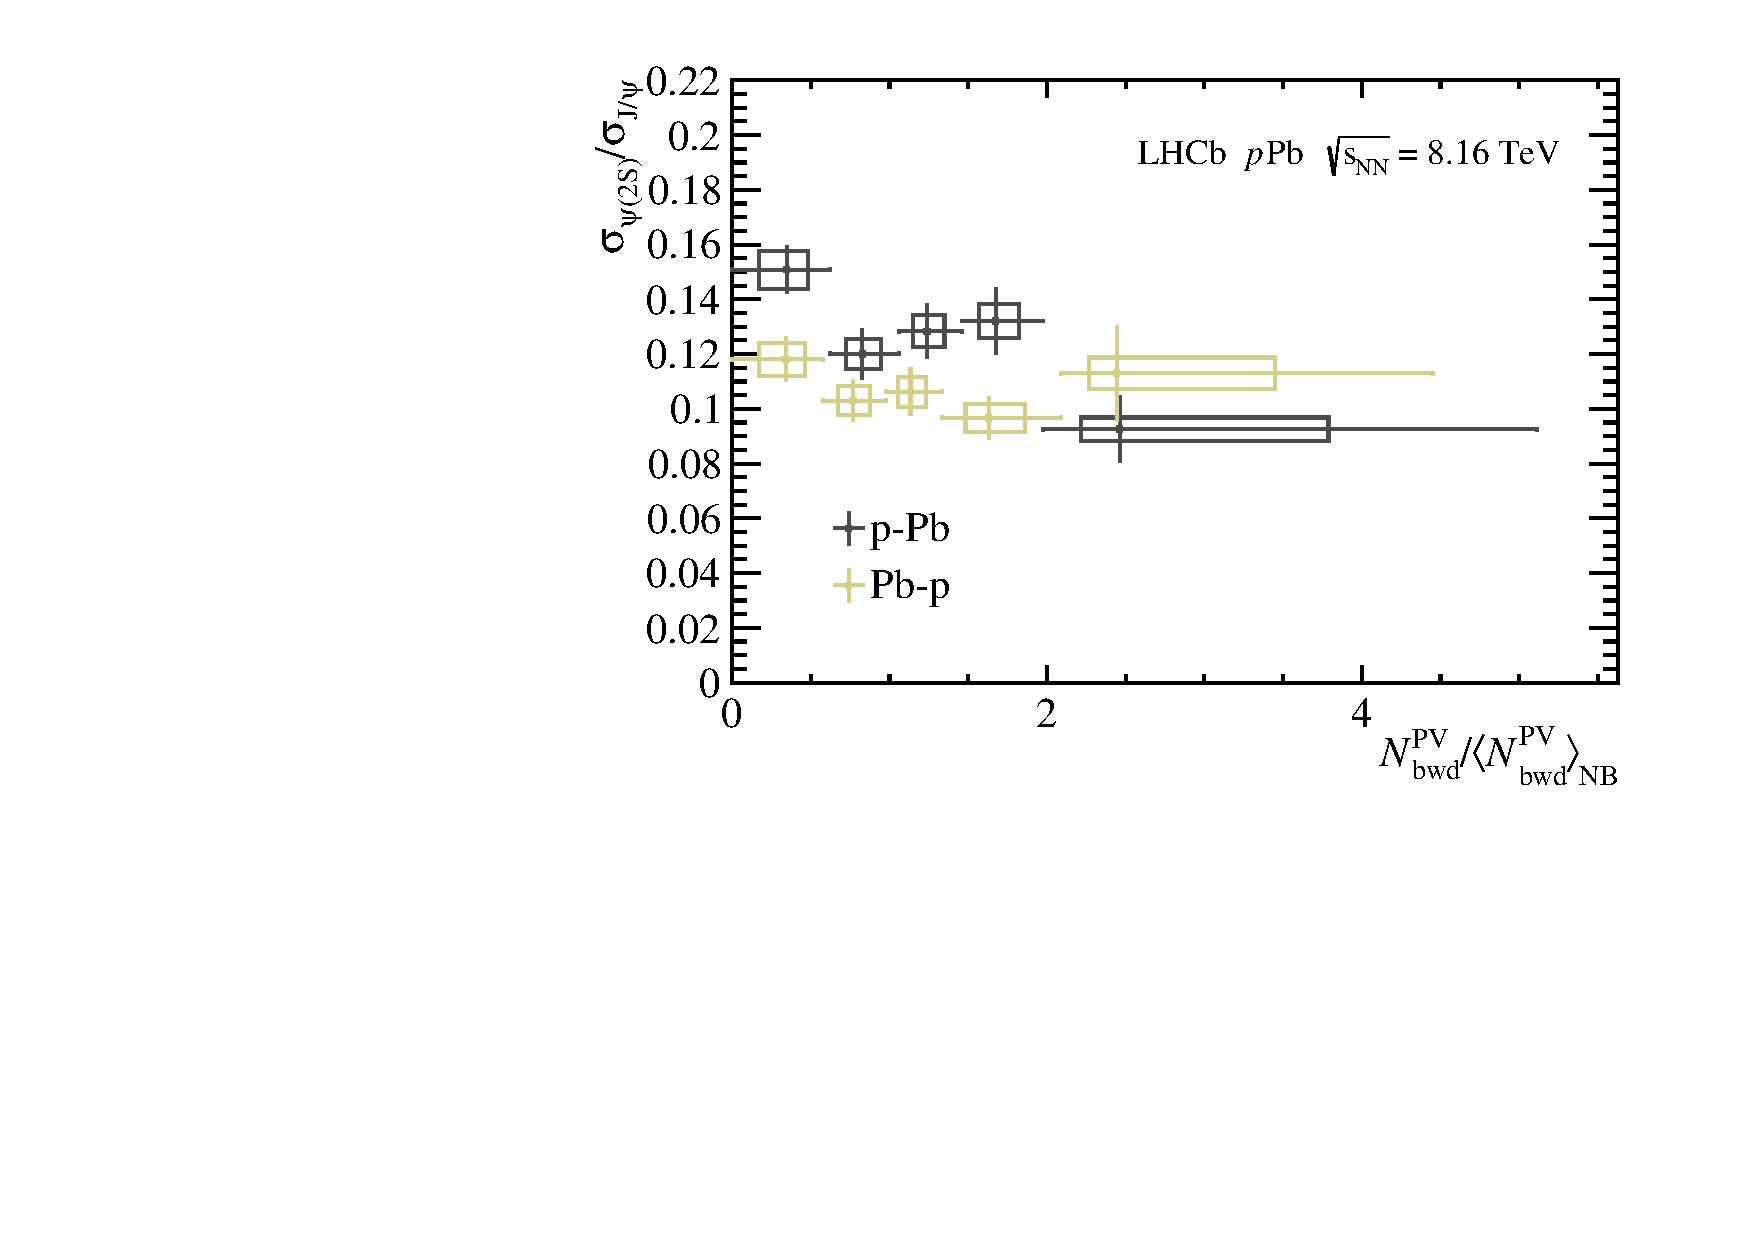
\includegraphics[width=0.7\linewidth]{pdf/pPb/BWorkdir/Result/Norm.pdf}
    \end{center}
    \caption{Prompt \psitwos-to-\jpsi production ratio compared with measurement in $pp$ collisions as a function of $N^{\rm PV}_{\rm bwd}$.
      }
    \label{RBackpp}
\end{figure}

